% This is a sample file for the Undergraduate Faculty Program at
% PCMI, containing one lecture 
%
%   What is a Partial Differential Equation?
%
%  from the Park City Lectures of Andrew J. Bernoff.
%
% The sample file illustrates the use of epsf.tex to include postscript 
% graphics, as well as various "AmS-LaTeX" constructions from the amsmath
% package (which is automatically loaded by the pcms-l document class).
% To run this file you need the files 
%
%        pcms-l.cls and pcmslmod.tex
%


\documentclass[lecture,12pt,]{pcms-l}
\input pcmslmod.tex  % v.1.2
%\input epsf.tex
\usepackage[framed,numbered,autolinebreaks,useliterate]{mcode}
\usepackage{graphicx}
\usepackage[toc,page]{appendix}
%\usepackage{natbib}
%\usepackage{amssymb} % this command would have loaded all the extra symbols,



% authors should not define these, they will be defined by the volume editors
%\def\currentvolume{3}
%\def\currentyear{1993}


% EQUATION NUMBERING AND THEOREM SETUP

\numberwithin{section}{chapter}
\numberwithin{equation}{chapter}

\theoremstyle{plain}
\newtheorem{theorem}[equation]{Theorem}
\newtheorem{lemma}[equation]{Lemma}

\theoremstyle{definition}
\newtheorem{example}{Example}[section]

\theoremstyle{definition}
\newtheorem{definition}[equation]{Definition}

\newtheorem{exercise}{Exercise}
\newtheorem{problem}{Problem}
\newtheorem*{remark}{Remark}

% Set enumerate to use letters, not numbers for problem parts.

\renewcommand{\theenumi}{\alph{enumi}}
\renewcommand{\labelenumi}{(\theenumi)}

% AUTHOR-DEFINED MACROS:

\newcommand{\cA}{\mathcal{A}}
\newcommand{\cB}{\mathcal{B}}
\newcommand{\C}{\mathbb{C}}
\newcommand{\cC}{\mathcal{C}}
\newcommand{\cD}{\mathcal{D}}

\begin{document}

\mainmatter
\setcounter{page}{1}

%\LogoOn

\lectureseries[Bayesian Analysis]{Decision Theory and Bayesian Analysis}


\auth[Dr. Vilda Purutcuoglu]{Dr. Vilda Purutcuoglu}
\address{Tubitak Space Technologies Research Institute, Ankara, 06800, Turkey}

\footnote{Edited by Anil A. Aksu based on lecture notes of STAT 565 course by Dr. Vilda Purutcuoglu }
%\email{ajb@hmc.edu}



% the following hack starts the lecture numbering at 1
\setcounter{lecture}{0}
\setcounter{chapter}{0}
\tableofcontents
%\listoffigures

\lecture{Bayesian Paradigm}

%\section{Outline of Lecture}
%\begin{itemize}
%\item{What is a Partial Differential Equation?}
%\item{Classifying PDE's: Order, Linear vs. Nonlinear}
%\item{Homogeneous PDE's and Superposition}
%\item{The Transport Equation} 
%\end{itemize}


\section{Bayes theorem for distributions}

If $A$ and $B$ are two events,
\begin{equation}
P(A\mid B)=\frac{P(A)P(B\mid A)}{P(B)}.
\end{equation}
This is just a direct consequence of the multiplication law of probabilities that says we can express $P(A\mid B)$ as either $P(A)P(B\mid A)$ or $P(B)P(A\mid B)$. For discrete distributions, if $Z,Y$ are discrete random variables
\begin{equation}
\label{eq:1}
P(Z=z\mid Y = y)=\frac{P(Z =z)P(Y = y\mid Z =z)}{P(Y = y)}.
\end{equation}
\begin{itemize}
\item How many distributions do we deal with here?
\end{itemize}
We can express the denominator in terms of the distribution in the numerator\cite{Allen}.
\begin{equation}
P(Y = y)=\sum_z P(Y = y, Z =z)=\sum_z P(Z= z)P(Y = y\mid Z =z).
\end{equation}
\begin{itemize}
\item This is sometimes called the law of total probability 
\end{itemize}
In this context, it is just an expression of the fact that as $z$ ranges over the possible values of $Z$
, the probabilities on the left hand-side of equation \ref{eq:1} make up the distribution of $Z$ given $Y=y$, and so they must add up to one. The extension to continuous distribution is easy. If $Z,Y$ are continuous random variable,
\begin{equation}
f(Z\mid Y)=\frac{f(Z)f(Y\mid Z)}{f(Y)}.
\end{equation}
where the denominator is now expressed as an integral:
\begin{equation}
f(Y)=\int f(Z)f(Y\mid Z)\mathrm{d}Z.
\end{equation}
\begin{equation}
f=
\left\{\begin{matrix}
continous \quad name ?\\ 
discrete \quad name ?
\end{matrix}\right.
\end{equation}


\vfill
%\begin{center}
%{\it (Room for notes)}
%\end{center}
\eject

\section{How Bayesian Statistics Uses Bayes Theorem}
\begin{theorem}[Bayes' theorem]
\label{Bayes}
\[P(A\mid B)=\frac{P(A)P(B\mid A)}{P(B)}\]
$P(B)$=if we are interested in the event $B$, $P(B)$ is the initial or prior probability of the occurence of event $B$. Then we observe event $A$ 
\\
$P(B\mid A)=$ How likely $B$ is when $A$ is known to have occurred is the posterior probability $P(B\mid A)$. 
\end{theorem}
Bayes' theorem can be understood as a formula for updating from prior to posterior probability, the updating consists of multiplying by the ratio $P(B\mid A)/P(A)$. It describes how a probability changes as we learn new information. Observing the occurrence of $A$ will increase the probability of $B$ if $P(B\mid A)>P(A)$.
From the law of total probability,
\begin{equation}
P(A)=P(A\mid B)P(B)+P(A\mid B^c)+P(A\mid B^c)P(B^c).
\end{equation}
where $P(B^c)=1-P(B)$.
\begin{lemma}
\[P(A\mid B)-P(A)=\frac{P(A)-P(A\mid B^c)P(B^c)}{1-P(B^c)}-P(A)\]
\end{lemma}
 
\begin{proof}
\[P(A\mid B)-P(A)=\frac{P(A)-P(A\mid B^c)P(B^c)-P(A)+P(A)P(B^c)}{P(B)}\]
\[P(A\mid B)-P(A)=\frac{P(B^c)(P(A)-P(A\mid B^c))}{P(B)}\]
\[P(A\mid B)-P(A)=P(B^c)(\frac{P(B)P(A\mid B)+P(B^c)P(A\mid B^c)}{P(B)}-\frac{P(A\mid B^c)}{P(B)})\]
\[P(A\mid B)-P(A)=P(B^c)(P(A\mid B)-\frac{P(A\mid B^c)(1-P(B^c))}{P(B)})\]
\[P(A\mid B)-P(A)=P(B^c)(P(A\mid B)-P(A\mid B^c))\]
\end{proof}
\subsection{Generalization of the Bayes' Theorem}
Let $B_1,...,B_n$ be a set of mutually exclusive events. Then
\begin{equation}
P(B_r\mid A)=\frac{P(B_r)P(A\mid B_r)}{P(A)}=\frac{P(B_r)P(A\mid B_r)}{\sum_{i=1}^n P(B_r)P(A\mid B_r)}.
\end{equation}
\begin{itemize}
\item Assuming that $P(B_r)>0$,$P(A\mid B)>P(A)$ if and only if $P(A\mid B)>P(A\mid B^c)$.
\item In Bayesian inference we use Bayes' theorem in a particular way.
\item $Z$ is the parameter (vector) $\theta$.
\item $Y$ is the data (vector) $X$.
\end{itemize}
So we have 
\begin{equation}
f(\theta\mid X)=\frac{f(\theta)f(X\mid \theta)}{f(X)}
\end{equation}
\begin{equation}
f(X)=\int f(\theta)f(X\mid \theta)\mathrm{d}\theta.
\end{equation}
\begin{equation}
f(\theta)=
\end{equation}
\begin{equation}
f(\theta\mid X)=
\end{equation}
\begin{equation}
f(X\mid \theta)=
\end{equation}
\subsection{Interpreting our sense} 
How do we interpret the things we see, hear, feel, taste or smell?
\begin{example}
I hear a song on the radio I identify the singer as Robbie Williams. Why do I think it's Robbie Williams?. Because he sounds like that. Formally, $P($ What I hear Robbie Williams $)>>P($What I hear someone else $)$
\end{example}
\begin{example}
I look out of the window and see what appears to be a tree. It has a big, dark coloured part sticking up out of the ground that branches into thinner sticks and on the ends of these are small green things. Clearly, $P(view \mid  tree)$ is high and $P(view \mid car)$ or $P(view \mid Robbie \quad Williams)$ are very small. But $P(view \mid carboard \quad cutout \quad cunningly \quad painted \quad to \quad look \quad like \quad a \quad tree)$ is also very high. Maybe even higher than $P(view \mid  tree)$ in the sense that what I see looks almost like a tree.
\\
Does this mean I should now believe that I am seeing a cardboard cut-out cunningly painted to look like a tree? No because it is much less likely to begin with than a red tree.
\end{example}
In statistical terms, consider some data $X$ and some unknown parameter $\theta$. The first step in any statistical analysis is to build a model that links the data to unknown parameters and the main function of this model is to allow us to state the probability of observing any data given any specified values of the parameters. That is the model defines $f(x\mid \theta)$. 
\\
When we think of $f(x\mid \theta)$ as a function of $\theta$ for fixed observed data $X$, we call it likelihood function and it by $L(\theta,X)$.
\begin{itemize}
\item So how can we combine this with our example?
\end{itemize}
This perspective underlies the differences between the two main theories of statistical inference.
\begin{itemize}
\item Frequentist inference essentially uses only the likelihood, it does not recognize $f(\theta)$.
\item Bayesian inference uses both likelihood and $f(\theta)$.
\end{itemize}
The principal distinguishing feature of Bayesian inference as opposed to frequentist inference is its use of $f(\theta)$.

\section{Prior to Posterior}
We refer to $f(\theta)$ as the \underline{prior distribution} of $\theta$. It represents knowledge about $\theta$ prior to observing the data $X$. We refer to $f(\theta \mid X)$ as the \underline{posterior distribution} of $\theta$ and it represents knowledge about $\theta$ after observing $X$. 
\begin{itemize}
\item So we have two sources of information about $\theta$.
\item Here $f(x)$ does not depend on $\theta$. Thus $\int f(\theta \mid x) \mathrm{d} \theta=1$. Since $f(x)$ is a constant within the integral, we can take it outside to get $1=f^{-1}(x)\int f(\theta) f(x \mid \theta) \mathrm{d}\theta$.
\item $f(\theta \mid x)= \propto f(\theta) f(x \mid \theta)\propto f(\theta) L(\theta ; x)$ (the posterior is proportional to the prior times the likelihood).
\item The constant that we require to scale the right hand side to integrate to $1$ is usually called the normalizing constant. If we haven't dropped any constants form $f(\theta)$ or $f(x \mid \theta)$, then the normalising constant is just $f^{-1}(x)$, otherwise it also restores any dropped constants. 
\end{itemize}
\section{Triplot}
If for any value of $\theta$, we have either $f(\theta)=0$ or $f(x\mid \theta)=0$, then we will also have $f(\theta \mid x)=0$. This is called the property of zero preservation. So if either:
\begin{itemize}
\item the prior information says that this $\theta$ value is impossible
\item the data say that this value of $\theta$ is impossible because if it were the true value, then the observed data would have been impossible, then the posterior distribution confirms that this value of $\theta$ is impossible.
\end{itemize}

\begin{definition}{Crowwell's Rule:}
If either information source completely rules out a specific $\theta$, then the posterior must rule it out too. This means that we should be very careful about giving zero probability to something unless it is genuinely impossible. Once something has zero probability then no amount of further evidence can cause it to have a non-zero posterior probability.
\end{definition}

\begin{itemize}
\item More generally, $f(\theta \mid x)$ will be low if either $f(\theta)$ is very small.  We will tend to find that $f(x \mid \theta)$ is large when both $f(\theta)$ and $f(x \mid \theta)$ are relatively large, so that this $\theta$ value is given support by \underline{both} information sources.
\end{itemize}
When $\theta$ is a scalar parameter, a useful diagram is the \underline{triplot}, which shows the prior, likelihood and posterior on the same graph. An example is in Figure \ref{fig:Triplot}.\footnote{All plots are generated in R, relevant codes are provided in Appendix R Codes }
\begin{figure}
\centering
 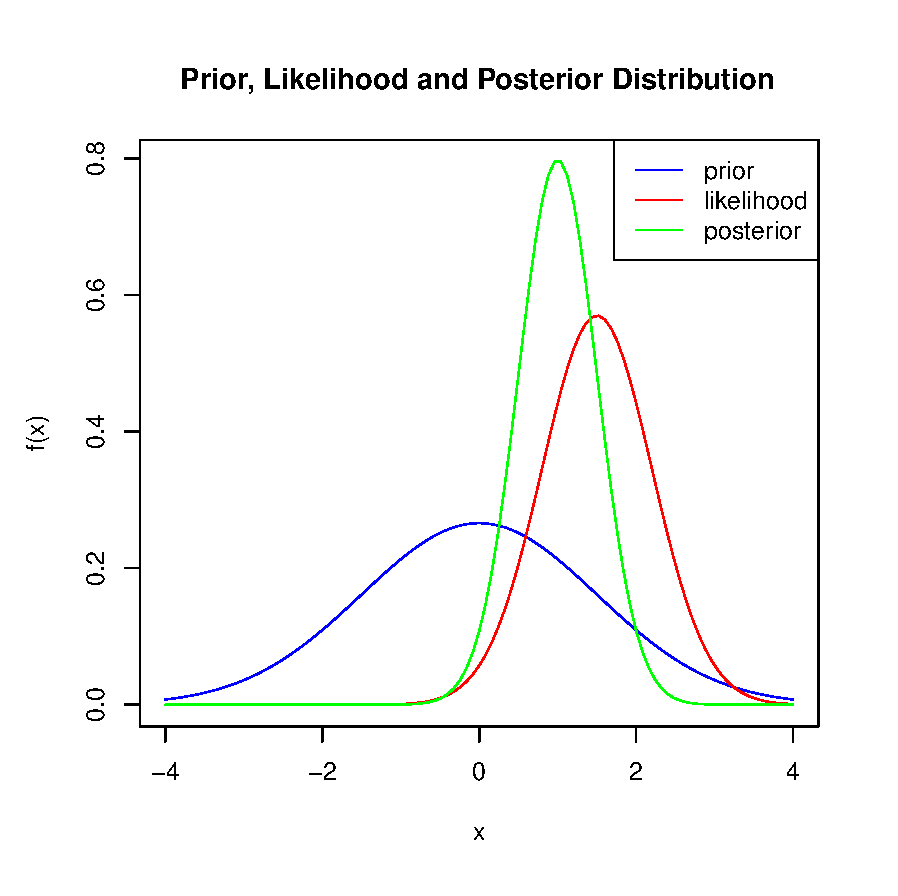
\includegraphics[scale=0.7]{triplot}% Images in 100% size
  \caption{Triplot of prior, likelihood and posterior. }
\label{fig:Triplot}
\end{figure} 
\\
\\
A strong information source in the triplot is indicated by a cırve that is narrow (and therefore, because it integrates to one, also has a high peak). A narrow curves concentrates on a small range of $\theta$ values, and thereby "rules out" all values of $\theta$ outside that range.

\vfill
\eject
\begin{itemize}
\item Over the range $\theta<-1$, the likelihood:
\item Over the range $\theta>3$,the likelihood:
\item Values of $\theta$ between $-1$ and $3$, the likelihood:
\item The maximum value of the posterior at:
\item The MLE of $\theta$ is:
\end{itemize}
\subsection{Normal Mean}
For example, suppose that $X_1, X_2,...,X_n$ are iid $ \mathcal{N}(\mu,\,\sigma^{2})$ and $\sigma^2$ is known. Then the likelihood is :
\begin{equation}
\begin{split}
f(x \mid \mu)= \prod_{i=1}^{n}f(x_i \mid \mu)=\prod_{i=1}^{n}\frac{1}{\sqrt{2\pi}\sigma}\exp\left (  -\frac{1}{2\sigma^2}(x_i -\mu)^2 \right )
\\
\propto \exp\left (  -\frac{1}{2\sigma^2}(x_i -\mu)^2 \right ).
\end{split}
\end{equation}
As,
\begin{equation}
\begin{split}
\sum (x_i-\bar{x}+\bar{x}-\mu)^2=\sum (x_i-\bar{x})^2+n(\bar{x}-\mu)^2+2(\bar{x}-\mu)\sum(x_i-\bar{x})
\\
=\sum (x_i-\bar{x})^2+n(\bar{x}-\mu)^2
\\
\propto \exp\left (  -\frac{1}{2\sigma^2}n(\bar{x} -\mu)^2 \right ).
\end{split}
\end{equation}
Note that $2(\bar{x}-\mu)\sum(x_i-\bar{x})=0$ as $\sum(x_i-\bar{x})=0$. Suppose the prior distribution for $\mu$ is normal:
\begin{equation}
\mu \sim \mathcal{N}(m,v).
\end{equation}
Then applying Bayes' theorem we have:
\begin{equation}
\begin{split}
f(\mu \mid x) \propto \underbrace{\exp\left (  -\frac{1}{2\sigma^2}n(\bar{x} -\mu)^2 \right )}_{f(x \mid \mu)} \underbrace{\exp\left (  -\frac{1}{2\sigma^2}n(\mu-m)^2 \right )}_{f(\mu)}
\\
=\exp\left (  -\frac{\theta}{2} \right ).
\end{split}
\end{equation}
Note that
\begin{equation}
\theta=n \sigma^{-2}(\bar{x}-\mu)+v^{-1}(\mu-m)^2=(v^*)^{-1}(\mu-m^*)^2+R
\end{equation}
and 
\begin{equation}
v^*=(n\sigma^{-2}+v^{-1})^{-1}
\end{equation}
\begin{equation}
m^*=(n\sigma^{-2}+v^{-1})^{-1}(n \sigma^{-2}\bar{x}+v^{-1}m)=a \bar{x}+(1-a)m 
\end{equation}
where $a=n \sigma^-2/(n \sigma^{-2}+v^{-1})$
\begin{equation}
R=(n^{-1}\sigma^2+v)(\bar{x}-m)^2
\end{equation}
Therefore,
\begin{equation}
f(\mu \mid x) \propto \exp\left (  -\frac{1}{2\sigma^2}n(\mu-m)^2 \right )
\end{equation}
and we have shown that the posterior distribution is normal too: $\mu \mid x \sim \mathcal{N}(m^*,\,v^*)$
\begin{itemize}
\item $m^*=$ weighted average of the mean $m$ and the usual frequentist data-only estimate $\bar{x}$. 
\\
The weights $\propto$:
\item Bayes' theorem typically works in this way. We \underline{usually} find that posterior estimates are compromises between prior estimates and data based estimates and tend to be closer whichever information source is stronger. And we \underline{usually} find that the posterior variance is smaller than the prior variance.
\end{itemize}
\subsection{Weak Prior Information}
It is the case where the prior information is much weaker that the data. This will occur, for instance, if we do not have strong information about $Q$ before seeing the  data, and if there are lots of data. Then in triplot, the prior distribution will be much broader and flatter that the likelihood. \underline{So the posterior is approximately proportional to the likelihood.}
\begin{example}
In the normal mean analysis, we get weak prior information by letting the prior precision of $v^{-1}$ become small. Then $m^* \rightarrow \bar{x}$ and $v^* \rightarrow \sigma^2/n$ so that the posterior distribution of $\mu$ corresponds very closely with standard frequentist theory.
\end{example}



\vfill
\eject




\lecture{Some Common Probability Distributions}

\lecture{Inference}

\appendix


\chapter*{Basic Statistics}

\chapter*{R Codes}

\lstinputlisting[caption={Triplot Code in R}]{BasicStatistics.R}

\bibliographystyle{plain}
% Note the spaces between the initials
\bibliography{Bayes}
\end{document}